% cours_info.tex

\documentclass[a4paper]{article}

\usepackage[french]{babel}
\usepackage{a4}
\usepackage[T1]{fontenc}	% pour les polices
\usepackage[utf8]{inputenc}	% encodage
\usepackage{graphicx}	% pour les images
\usepackage{epsfig}	% pour les images au format PostScript
\usepackage{float}	% pour le placement des images
\usepackage{version}	% pour pouvoir faire des commentaires sur plusieurs lignes avec \begin{comment}
						% et \end{comment}
\usepackage[a4paper,left=3cm,right=3cm,top=2cm,bottom=2cm]{geometry}	% pour pouvoir régler les marges
\usepackage{listings}	% Pour inclure du code ; Cf http://www.ctan.org/tex-archive/help/Catalogue/entries/listings.html
\lstset{language=C++}

\begin{document}

\begin{center}

\includegraphics[width=16cm]{images/logos.png}
\Huge{\textbf{Introduction à l'informatique au club robot\\}}
\vspace{3cm}
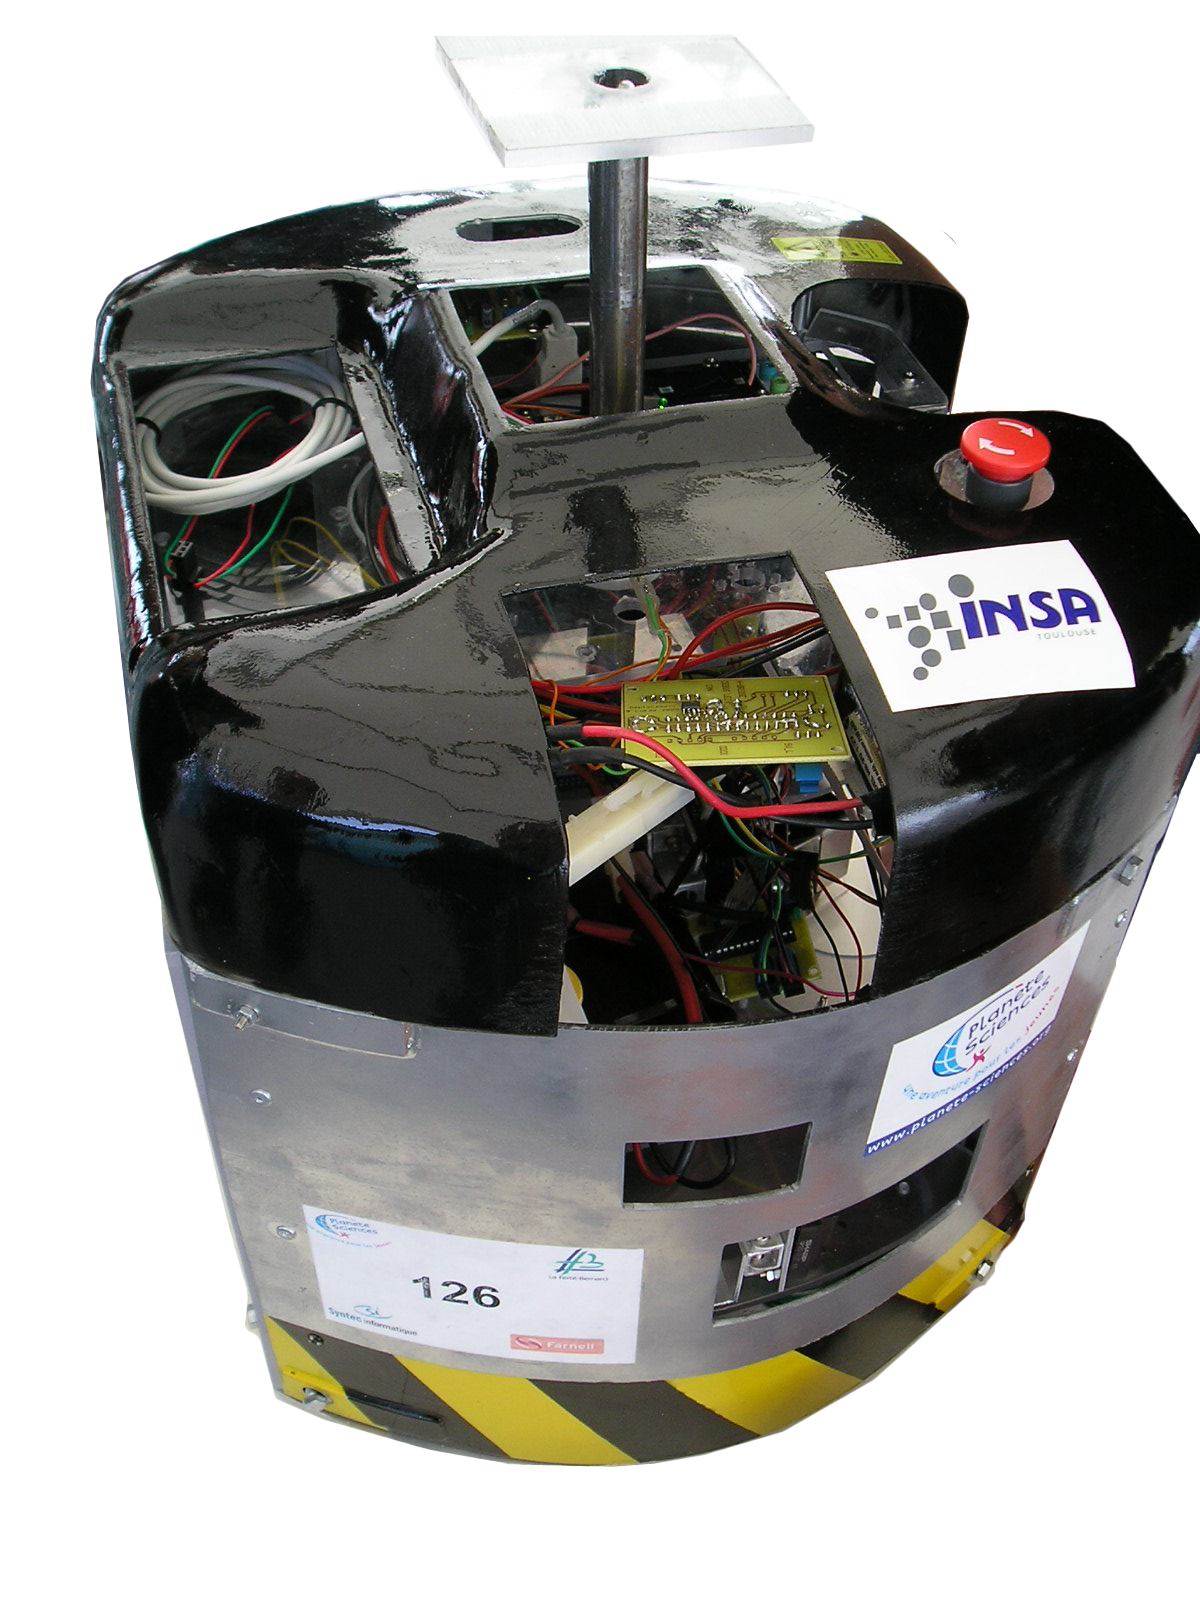
\includegraphics[width=7cm]{images/pandora.png}
\end{center}

\newpage

\textbf{Introduction}\\

Ce document a pour but de résumer ce qu'il est nécessaire de savoir pour pouvoir travailler sur la partie informatique du robot. Il vise surtout à vous présenter ce qui a déjà été fait, comment cela a été réalisé et quelles sont les perspectives pour cette année (2009).

\tableofcontents

\include{introduction}
% 1_environnement.tex

\section{Environnement de développement}

Pour développer sur le robot, on peut utiliser au choix un système Windows ou un système GNU/Linux ; d'autres plate-formes peuvent s'ajouter simplement, on n'en a juste pas eu la nécessité jusque là.\\
Au niveau de ce qu'il vous est nécessaire pour pouvoir développer quelque chose, il y a :\\
\begin{itemize}
\item \textbf{Un compilateur} : Sous Linux, g++ s'impose, et sous Windows je vous conseillerais d'utiliser son portage, "MinGW", avec l'environnement Code::Blocks (Cf les liens). Bien évidemment, n'importe quel environnement convient, faites comme bon vous semble :) Au niveau de l'intégration avec un environnement existant, il peut être pratique de passer par un Makefile qui appelle SCons ; par exemple, avec Code::Blocks, on peut lui spécifier d'utiliser un Makefile personnalisé. De tels Makefiles sont sur le serveur SVN.\\
\item \textbf{SVN} : un client SVN est indispensable pour pouvoir récupérer une copie du dépôt du club. SVN est un système de gestion de version, qui permet dans un projet à plusieurs d'avoir un serveur central qui contienne les fichiers sur lesquels on travaille. L'avantage d'un tel système de gestion de version par rapport à un simple compte FTP par exemple est qu'il permet de garder plusieurs versions d'un même fichier, et qu'un update sur votre copie ne téléchargera que les différences, par exemple. Sous GNU/Linux, vous pouvez utiliser le client en ligne de commande, ou bien RapidSVN ou eSVN ; sous Windows, le client le plus connu et le plus utilisé est TortoiseSVN. Des explications sont données sur le Trac du club (Cf les liens à la fin de ce document).\\
\item \textbf{SCons} : \textbf{S}oftware \textbf{Cons}truction tool : il s'agit du système que l'on utilise pour compiler toute la partie informatique du robot. C'est un équivalent aux classiques Makefiles et autotools de UNIX, mais bien mieux pensé. On crée des fichiers du nom de \texttt{SConstruct}, qui contiennent du code dans le langage interprété \texttt{Python}. Un mini-tuto sur son utilisation est disponible sur le Trac, il s'appuie sur le didacticiel plus général qui se trouve ici : \begin{verbatim}http://www.coder-studio.com/?page=tutoriaux_aff&code=autre_5\end{verbatim} .\\
\item \textbf{pthreads-win32} : \underline{seulement} pour les utilisateurs de Windows : cette librairie est un portage Windows de la librairie standard "pthreads" de UNIX. Elle sert à faire de la programmation en multithreading, i.e. de permettre d'avoir plusieurs fonctions qui s'exécutent en parallèle. Elle est utilisée par la libRobot, entre-autres.\\
\item \textbf{Dépendances sous GNU/Linux : libxrandr, libbluetooth, Mesa3D, libv4l} : \underline{seulement} pour les utilisateurs de GNU/Linux : libxrandr et Mesa3D sont utilisés par GLFW (Cf plus loin), libbluetooth est nécessaire pour la libcwiimote (Cf plus loin aussi) et libv4l pour la libWebcam. Sur une Debian ou une Ubuntu, les paquets à installer sont \texttt{libxrandr-dev}, \texttt{libbluetooth-dev}, \texttt{libgl1-mesa-dev}, \texttt{libglu1-mesa-dev} et \texttt{libv4l-dev}.\\
\\
\end{itemize}

Les autres librairies sont normalement déjà inclues dans les fichiers du dépôt SVN :\\
\begin{itemize}
\item \textbf{GLFW} : Open\textbf{GL} \textbf{F}rame\textbf{W}ork : utilisée dans le simulateur, le programme de debug au clavier, le programme de test de la webcam...etc ; c'est une librairie qui permet d'ouvrir facilement une fenêtre utilisant OpenGL et d'utiliser le clavier et la souris. Elle sera utile pour ceux qui voudront développer des applications graphiques (programmes de debug pour les électroniciens par exemple).\\
\item \textbf{Bullet} : moteur physique utilisé par le simulateur\\
\item \textbf{libcwiimote} : \underline{seulement} pour les utilisateurs de GNU/Linux : c'est la librairie qui permet d'utiliser une wiimote, pour contrôler le robot par exemple :)\\
\end{itemize}

% 2_cplusplus.tex

\section{Un peu de C++...}

Cette section a été écrite pour ceux qui ne connaissent absolument pas le C++ et les concepts de la programmation orientée objets (POO).\\
Pour ceux qui ne connaissent que le C, ça peut être utile aussi :)\\
C'est un résumé \underline{très, très} loin d'être exhaustif, et qui suppose que vous ayiez un minimum de connaissances en programmation (disons, UV1 de 1\up{ère} année d'Ada :)). C'est plus un résumé, un aide-mémoire qu'autre chose, et les notions y sont assez expédiées ^^ Le but est que vous soyiez capables de lire et de modifier du code écrit par les membres du club, et de progresser ensuite par vous-mêmes. Voici donc pour commencer le classique Hello World :

\begin{lstlisting}
// Hello World :

#include <stdio.h>	// On inclut la librairie standard d'input/output

// Fonction principale, "main()" : c'est la 1ere a etre appelee.
int main()	// Elle renvoie un entier (int), code de retour du programme.
{
	printf("Hello World !\n");	// Affichage d'un message a l'ecran.
	return 0;	// Valeur de retour de la fonction main(),
				// qui est la valeur de retour du programme.
}
\end{lstlisting}

\begin{itemize}
\item Les commentaires débutent par "//" (une seule ligne) ou sont encadrés par "/*" et "*/" (commentaires sur plusieurs lignes).\\

\item \lstinline{#include} : la ligne "\lstinline{#include <stdio.h>}" est remplacée à la compilation par le contenu du fichier "stdio.h", qui se trouve dans \texttt{/usr/include} sous UNIX et dans le répertoire de votre compilateur sous Windows (ex : C:$\backslash$CodeBlocks$\backslash$MinGW$\backslash$include). Ce travail est effectué par un programme particulier, le "préprocesseur", qui interprète toutes les lignes débutant par un "\#". C'est la première chose qui est effectuée, après le retrait des commentaires, à la compilation. Pour inclure un fichier .h se trouvant dans le même répertoire que le fichier source où est écrit le "\lstinline{#include}", on utilisera \lstinline{#include "mon_header.h"} plutôt que \lstinline{#include <mon_header.h>}\\

\item \lstinline{#define} : autre commande du préprocesseur, elle s'utilise en général pour définir une constante (mais permet de faire beaucoup plus :)). Toutes les occurences dans le code du symbole défini seront remplacées par la chaîne de caractères indiquée. Exemple :\\
\lstinline{#define MA_CONSTANTE 42}\\
Tous les endroits dans le code où l'on verra écrit "MA\_CONSTANTE" seront remplacés par "42".

\item Déclaration d'une variable : \lstinline{type nom_variable;} ; exemple :\\
\lstinline{int var;}\\
Une variable peut être déclarée n'importe où dans une fonction (variable locale), ou même en dehors (variables globales), auquel cas la variable est utilisable partout dans le code. C'est une \textbf{très mauvaise pratique} car cela désorganise totalement le code, le rendant difficile à relire et à faire évoluer.\\
Souvenez-vous de ceci : "\textit{Global, c'est mal, local, c'est génial !}".

\item Types de base pour les variables :
	\begin{itemize}
	\item \lstinline{bool} : valeur booléenne, valant soit \lstinline{true}, soit \lstinline{false} (\lstinline{Boolean} en Ada)
	\item \lstinline{char} : caractère (8 bits) (\lstinline{Character} en Ada) ; peut servir pour stocker simplement un octet, qui ne soit pas forcément un caractère.
	\item \lstinline{short} : nombre entier (16 bits)
	\item \lstinline{int} : nombre entier (32 bits) (\lstinline{Integer} en Ada)
	\item \lstinline{float} : nombre flottant (32 bits) (\lstinline{Float} en Ada)
	\item \lstinline{double} : nombre flottant double précision (64 bits)\\
	\end{itemize}
On peut rajouter l'attribut \lstinline{unsigned} devant \lstinline{int}, \lstinline{short} ou \lstinline{char} pour préciser que ce sont des nombres non signés, toujours positifs.

\item \lstinline{printf} : affichage d'un message sur la console : exemple :\\
\begin{lstlisting}
int var = 2;
printf("Message : %d %f %s %c", var, 4.2, "pouet", 'K');
// Affiche sur la console le message : "Message : 2 4.2 pouet K"
\end{lstlisting}
Le code spécial \%d sert à afficher un int, \%f à afficher un float, \%s une chaîne de caractères, \%c un caractère. La fonction \lstinline{printf} est déclarée dans le fichier stdio.h.\\

\item Opérations particulières sur les nombres :
\begin{lstlisting}
int i=0;
i++;	// Equivalent a "i = i+1;"
i++;	// Equivalent a "i = i-1;"
i+=3;	// Equivalent a "i = i+3;"
i%=2;	// Equivalent a "i = i%2", avec l'operateur % signifiant "modulo".
		// On met dans i le reste de la division entiere de i par 2.
\end{lstlisting}

\item \lstinline{if, for, while} : exemple :\\
\begin{lstlisting}
int i=0;
for(i=0 ; i<5 ; i++)
{
	if(i % 2 == 0)
		printf("%d ", i);
}

while(i > 0)
{
	printf("%d ", i);
	i--;
}

\end{lstlisting}
Un if, un for ou un while peuvent ne pas être suivis d'un bloc (i.e. du code entre { et }), auquel cas seule l'instruction qui suit est concernée. Ici, par exemple, le if n'est pas suivi d'un bloc car il n'y a qu'une seule instruction, qui est l'appel à printf(). On aurait aussi bien pu écrire :\\
\begin{lstlisting}
for(i=0 ; i<5 ; i++)
	if(i % 2 == 0)
	{
			printf("%d ", i);
	}
\end{lstlisting}

\item Tableaux : \\
\begin{lstlisting}
int tab[5] = {1, 2, 3, 4, 5};	// Tableau de 5 nombres entiers
tab[0] = 42;	// NB : contrairement a Ada, les indices d'un tableau
				// varient toujours entre 0 et sa taille -1 (ici 4).
\end{lstlisting}

\item Pointeurs : un pointeur est un type particulier de variable qui contient l'\underline{adresse} d'une autre variable.\\
\begin{itemize}
\item Déclaration : \lstinline{type* pointeur;}
\item Adresse mémoire d'une variable : \lstinline{&variable}
\item Valeur de la variable pointée par "pointeur" : \lstinline{*pointeur}\\
\end{itemize}
Exemple : \\
\begin{lstlisting}
int* pointeur;	// Pointeur qui n'est theoriquement capable
				// de pointer que sur des variables entieres
int var = 0;
pointeur = &var;	// Je mets dans pointeur l'adresse memoire de "var".
					// On dit que "pointeur pointe sur var".
*pointeur = 42;	// Je mets la valeur 42 dans la variable pointee par pointeur,
				// c'est a dire dans var.
printf("%d\n", var);	// Affiche 42
\end{lstlisting}

\item Déclaration/implémentation de fonctions : exemple :\\
\begin{lstlisting}
int carre(int a);	// Prototype de ma fonction, qui prend un entier "a" en entree et renvoie un entier.
int carre(int a)	// Implementation de ma fonction
{
	return a*a;	// Valeur de retour
}
// ...plus loin dans le code :
int var = carre(2);	// "var" vaut 4
\end{lstlisting}
Le prototype d'une fonction permet juste d'indiquer que la fonction "existe", tandis que son implémentation sert à indiquer ce qu'effectue réellement la fonction. En général, on place les prototypes dans des fichiers .h que l'on inclut ensuite, et les implémentations dans des fichiers .cpp.\\
Le type de retour spécial "void" signifie que la fonction ne renvoie pas de valeur. La fonction est alors équivalente à une "procedure" en Ada.

\item Classe/structure : équivalent du record en Ada. C'est la base de la programmation orientée objets. Une classe est un type particulier de variable, que l'on définit soit-même. Une variable dont le type est une classe est appelée "objet". Une classe peut contenir des variables dites "membres" ou "attributs", ainsi que des fonctions, dites aussi "méthodes". Exemple :\\
\begin{lstlisting}
class MaClasse
{
private:
	int a;
public:
	int b;
	void afficher()
	{
		printf("a == %d, b == %d\n", a, b);	// NB : '\n' est le caractere de retour a la ligne.
	}
};

// ...plus loin dans le code :
MaClasse objet;
printf("%d\n", objet.a);	// NE COMPILE PAS car MaClasse::a est en private
printf("%d\n", objet.b);	// OK
objet.afficher();	// Affiche les valeurs de a et de b
\end{lstlisting}

\item Héritage : l'héritage consiste à créer une nouvelle classe, dite "dérivée", à partir d'une classe dite "de base" ; la nouvelle classe "hérite" de tous les attributs et de toutes les variables membres de la classe de base. Ce mécanisme est équivalent à une recopie de la classe de base, à laquelle on ajoute de nouvelles fonctionnalités spécifiques à la classe dérivée. Exemple :\\
\begin{lstlisting}
class Base
{
public:
	void pouet()
	{
		printf("pouet !\n");
	}
};

class Derivee : public Base
{
public:
	void youpi()
	{
		printf("youpi !\n");
	}
};

// ...plus loin dans le code
Derivee objet;
objet.pouet();	// Affiche "pouet !"
objet.youpi();	// Affiche "youpi !"
\end{lstlisting}

\end{itemize}

% 3_architecture_robot.tex

\section{Architecture du robot}

\begin{center}
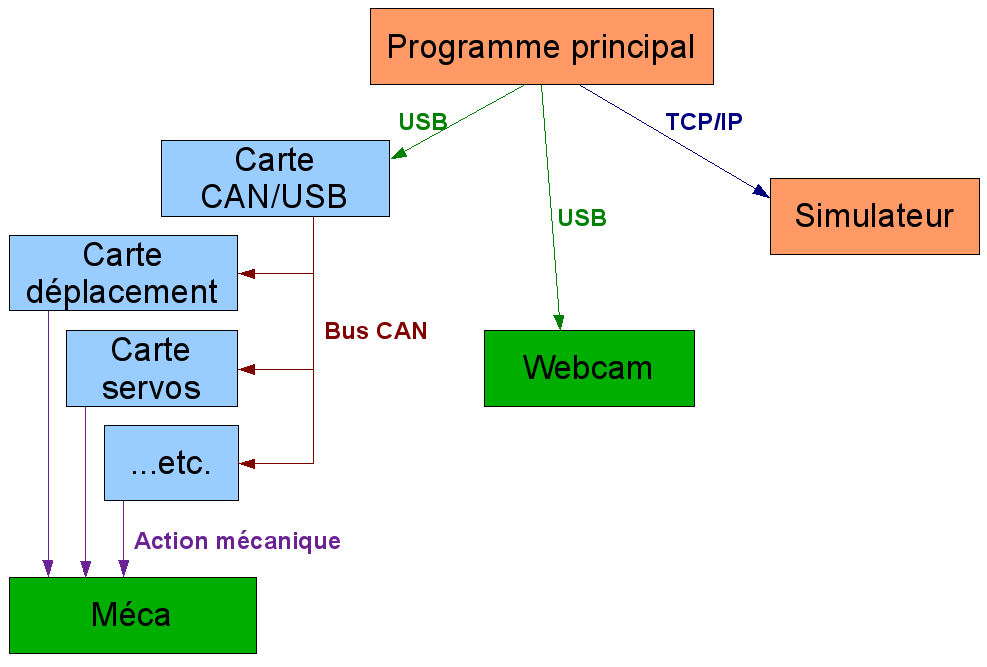
\includegraphics[width=12cm]{images/architecture_1.png}\\
\end{center}
\indent Le robot s'articule en 3 grandes parties : l'informatique, l'électronique et la mécanique. Le programme principal, linké avec les librairies nécessaires (libRobot, libRobot2008, libWebcam...), pilote soit le simulateur par TCP/IP, soit les cartes électroniques, qui elles-mêmes actionnent des servos, des moteurs...etc et pour faire agir le robot. Les cartes électroniques permettent aussi de renvoyer de l'information au programme principal, comme une position sur le terrain, si le robot a une balle à l'intérieur...etc.\\

\begin{center}
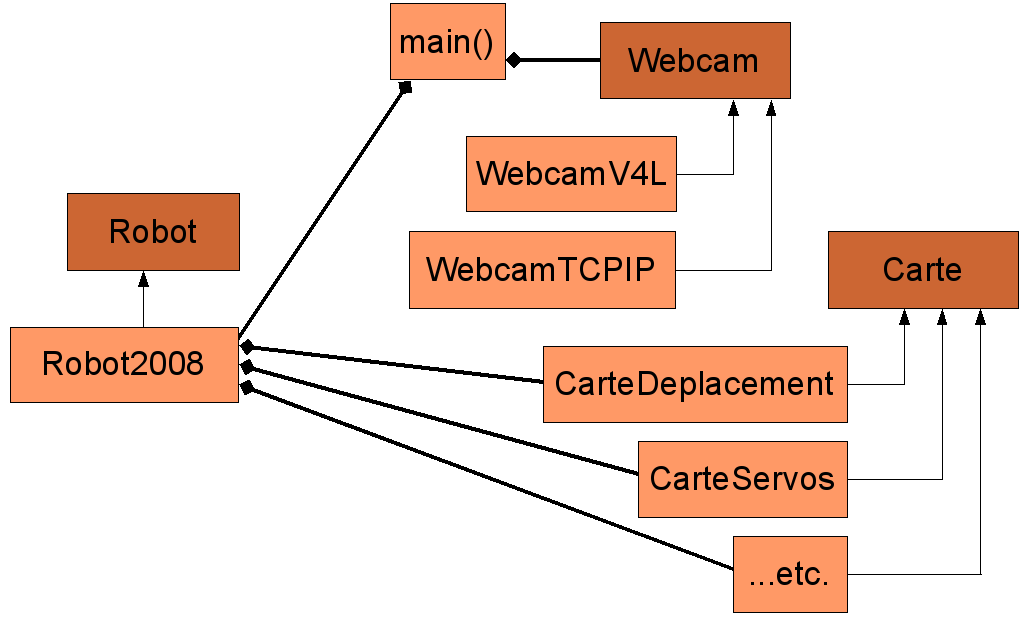
\includegraphics[width=12cm]{images/architecture_2.png}\\
\end{center}
\indent Au niveau de l'organisation des classes, le programme principal, main(), possède 2 instances des classes Robot2008 et WebcamV4L ou WebcamTCPIP. En réalité, le programme principal ne manipule qu'un pointeur Webcam*, la classe Webcam étant une interface permettant de piloter de façon transparente la véritable webcam, via l'API Video4Linux, ou la webcam du simulateur (communication par TCP/IP).\\
\indent La classe Robot2008 dérive de la classe Robot, qui sert de base aux robots de 2007, 2008...etc. Même chose pour les classes représentant les cartes, qui dérivent de la classe générale "Carte". Chaque carte expose une interface permettant de piloter les vraies cartes électroniques. Les instances des cartes appartiennent à Robot2008.\\
En plus clair, cela donne lieu à du code comme ceci :
\begin{lstlisting}
int main(int argc, char* argv[])
{
	Robot2008* robot = NULL;

	// Creation du robot
	if(!creationRobot(&robot, argc, argv))
		return -1;

	robot->initialiser();
	robot->getCarteDeplacement()->avancer(100);
	delete robot;
	return 0;
}
	
\end{lstlisting}

La fonction creationRobot() fait un "\lstinline{new Robot2008()}" (équivalent C++ d'un "\lstinline{malloc(sizeof(Robot2008))}" en C), puis règle certains paramètres pour la carte de déplacement, concernant les vitesses à utiliser. En fonction de ce qui est passé en argument au programme à son lancement, il communiquera soit par TCP/IP (avec le simulateur par exemple), soit par RS232 (avec le vrai robot en général).
% 4_projets.tex

\section{Projets}

\subsection{Projets utiles pour la coupe}
\begin{itemize}
\item Stratégies des matchs et réorganisation : pour l'année à venir, il nous faudra programmer une, ou plutôt plusieurs, nouvelle IA. Plusieurs IAs car on n'est jamais sûr à l'avance de ce qui fonctionnera ou pas le jour de la coupe, et de la configuration du terrain, de l'adversaire...etc. Il est prévu de programmer des IAs très basiques, et d'autres plus complexes, le choix se faisant le jour de la coupe. De même, il faudra réorganiser un petit peu le code pour les IAs, en faisant par exemple une classe de base RobotIA de laquelle pourront dériver toutes les IAs.\\
\item Interfaçage Info/Elec (cartes) : mettre à jour les cartes existantes si besoin est, revoir un peu la communication avec la carte déplacement, ajouter de nouvelles classes de cartes si besoin est.\\
\item Administration du système Linux embarqué ; il est prévu de tester l'installation d'une distribution Debian minimale sur le robot, pour ne plus avoir de problèmes avec la reconnaissance de la caméra, d'une clef bluetooth, d'une clef Wi-Fi...\\
\item Simulateur 3D : il devra être mis à jour avec les règles de cette année (modèles 3D de la table et du robot, gestion de la physique pour l'empilement...) et être tenu à jour au niveau des cartes simulées. Il est prévu de donner la possibilité à l'IA de demander un affichage particulier sur le simulateur, pour pouvoir par exemple afficher la "zone interdite" lors du calcul de l'algorithme A* (recherche du plus court chemin)\\
\item Webcam, reconnaissance d'objets : il faut adapter le code existant pour qu'il utilise la totalité de la résolution et non 1/4 de celle-ci. On pourrait aussi travailler sur l'application de filtres avec des matrices, pour détecter des contours, ou toute autre technique plus évoluée (pourquoi pas essayer de se repérer sur le terrain en utilisant les bords de celui-ci par exemple ? Ou, plus réaliste, essayer de détecter le robot adverse avec la webcam ?).\\
\item Interfaçage Python : en interfaçant l'API du robot avec le langage Python, on pourrait tester nos fonctions sans avoir besoin de recompiler, directement au prompt, ce qui serait un avantage notable. Les IAs pourraient ensuite être écrites en Python. En poussant plus loin, on pourrait faire un programme graphique où l'on définisse à la souris les déplacements que doive effectuer le robot :) Voire intégrer ça dans le simulateur...Bref, "moderniser" un peu notre approche :)\\
\item Programmes de debug pour les élecs : par exemple, en 2007, un programme de debug pour la carte de déplacement permettait de lui donner des ordres graphiquement et de voir où elle pensait se trouver sur le terrain.\\
\item Correction de fautes d'orthographe et réorganisation de certaines parties du projet...\\
\end{itemize}

\subsection{Projets moins utiles pour la coupe mais funs}
\begin{itemize}
\item Contrôle à la wiimote\\
\item Reconnaissance/synthèse vocale : faire parler le robot, le faire obéir à la voix !\\
\item Streaming vidéo : pouvoir piloter le robot à distance et voir ce qu'il voit sur notre PC :)\\
\item Carte LEDs : trouver de nouvelles combinaisons, l'interfacer avec la wiimote\\
\item ...etc\\
\end{itemize}
% liens.tex

\section{Liens}
\begin{itemize}
\item \textbf{Trac} : \begin{verbatim}https://www.etud.insa-toulouse.fr/trac/roboinsat\end{verbatim}
\item \textbf{SVN} : \begin{verbatim}https://svn.etud.insa-toulouse.fr/roboinsat\end{verbatim}
\item \textbf{Forum} : \begin{verbatim}https://www.etud.insa-toulouse.fr/~club_rob/forum\end{verbatim}
\item \textbf{Site web du club} : \begin{verbatim}https://www.etud.insa-toulouse.fr/~club_rob/joomla\end{verbatim}
\item \textbf{Code::Blocks} : \begin{verbatim}http://www.codeblocks.org\end{verbatim}
\item \textbf{libcwiimote} : \begin{verbatim}http://libwiimote.sourceforge.net\end{verbatim}
\item \textbf{pthreads-win32} : \begin{verbatim}http://sources.redhat.com/pthreads-win32/\end{verbatim}
\item \textbf{GLFW} : \begin{verbatim}http://glfw.sourceforge.net\end{verbatim}
\item \textbf{Tutorial SCons} : \begin{verbatim}http://www.coder-studio.com/?page=tutoriaux_aff&code=autre_5\end{verbatim}
\end{itemize}

\end{document}
